\documentclass[11pt]{article}


\usepackage[margin=1in]{geometry} 
\usepackage{amsmath,amsthm,amssymb,amsfonts}
\usepackage[utf8]{inputenc}
\usepackage[T1]{fontenc}
\usepackage{microtype}
\usepackage{mathpazo}
\usepackage{euler}
\usepackage{xcolor}
\usepackage{tikz}
\usepackage{tikz-cd}
\usetikzlibrary{arrows}
\usetikzlibrary{matrix}
\usepackage{fancyhdr}
\pagestyle{fancy}
\usepackage{enumitem}

\newcommand{\N}{\mathbb{N}}
\newcommand{\Z}{\mathbb{Z}}
\newcommand{\Q}{\mathbb{Q}}
\newcommand{\R}{\mathbb{R}}
\newcommand{\C}{\mathbb{C}}
\newcommand{\D}{\mathbb{D}}
\newcommand{\Ss}{\mathbb{S}}
\newcommand{\eps}{\varepsilon}
\newcommand{\tint}[1]{#1^o}
\newcommand{\nat}[1]{[\![#1]\!]}
\newcommand{\natzero}[1]{\nat{#1}_0}
\newcommand{\diam}[1]{\operatorname{diam}(#1)}
\newcommand{\rg}{\operatorname{rg}}
\newcommand{\im}{\operatorname{im}}
\newcommand{\tr}{\operatorname{tr}}
\newcommand{\cat}[1]{\mathsf{#1}}

\definecolor{color}{RGB}{31, 127, 0}
\newcommand{\paint}[1]{\color{color}{#1}}

\renewcommand*{\proofname}{\paint{Demostraci\'on}}
\newenvironment{theorem}[2][Teorema]{\begin{trivlist}
\item[\hskip \labelsep {\bfseries #1}\hskip \labelsep {\bfseries #2.}]}{\end{trivlist}}
\newenvironment{lemma}[2][Lema]{\begin{trivlist}
\item[\hskip \labelsep \paint{{\bfseries #1}}\hskip \labelsep {\bfseries #2.}]}{\end{trivlist}}
\newenvironment{exercise}[2][Ejercicio]{\begin{trivlist}
\item[\hskip \labelsep \paint{{\bfseries #1}}\hskip \labelsep {\bfseries #2.}]}{\end{trivlist}}
\newenvironment{reflection}[2][Resoluci\'on]{\begin{trivlist}
\item[\hskip \labelsep {\bfseries #1}\hskip \labelsep {\bfseries #2.}]}{\end{trivlist}}
\newenvironment{proposition}[2][Proposici\'on]{\begin{trivlist}
\item[\hskip \labelsep \paint{{\bfseries #1}}\hskip \labelsep {\bfseries #2.}]}{\end{trivlist}}
\newenvironment{corollary}[2][Corolario]{\begin{trivlist}
\item[\hskip \labelsep {\bfseries #1}\hskip \labelsep {\bfseries #2.}]}{\end{trivlist}}
\newenvironment{obs}[2][Observaci\'on]{\begin{trivlist}
\item[\hskip \labelsep \paint{{\bfseries #1}}\hskip \labelsep {\bfseries #2.}]}{\end{trivlist}}

%-----------------------

\title{
\LARGE{\paint{Topolog\'ia Algebraica}}
\\
\vspace{5pt}
\small{\paint{Ejercicios para Entregar - Pr\'acticas 4 y 5}}
\\
\vspace{5pt}
\large{\paint{Guido Arnone}}
\\
\paint{
\rule{250pt}{0.5pt}
}
}
\author{}
\date{}
\lhead{Guido Arnone}
\rhead{Pr\'acticas 4 y 5}

\begin{document}

\maketitle

\begin{center}
\paint{\large{Sobre los Ejercicios}}
\end{center}
\begin{center}

$\paint{
\rule{400pt}{0.5pt}
}$
\vspace{45pt}
\end{center}

\begin{obs}{1} Si notamos $I : \cat{Top} \to \cat{hTop}$ al funtor que es la identidad en objetos y envía cada función continua a su clase de homotopía, para cada espacio topológico $X$ tenemos un funtor al componer con $\cat{hTop}(X,-)$, 
\begin{center}
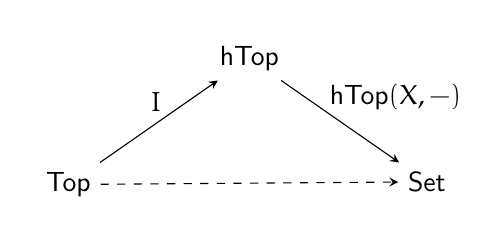
\begin{tikzpicture}
  \matrix (m) [matrix of math nodes,row sep=3em,column sep=4em,minimum width=2em]
  {
     & \cat{hTop} &\\
     \cat{Top} &  & \cat{Set} \\};
  \path[-stealth]
    (m-2-1) edge [dashed] node [above] {} (m-2-3)
    (m-2-1) edge node [above] {$I \ $} (m-1-2)
    (m-1-2) edge node [above] {$\quad \quad \quad \quad \cat{hTop}(X,-)$} (m-2-3);
\end{tikzpicture}
\end{center}
Concretamente, éste envía cada espacio $Y$ a $[X,Y]$ y cada función continua $f : Y \to Z$ a
\begin{align*}
[f]_* : [h] \in [X,Y] \mapsto [fh] \in [X,Z].
\end{align*}
En particular, si $f$ es una equivalencia homotópica entonces $If$ es un isomorfismo y por lo tanto así lo es $[f]_*$.
\end{obs}

\begin{lemma}{2} Sea $(X,A)$ un CW-par y $(Z,Y)$ un par topológico tal que $\pi_n(Z,Y) = 0$ para todo $n \geq 1$. Si $f : (X,A) \to (Z,Y)$ es una función continua de pares, entonces existe otra función continua $g : X \to Z$ tal que $g(X) \subset Y$ y $f \simeq g$ relativa a $Y$.
\end{lemma}
\begin{proof}

\end{proof}

\begin{exercise}{4} Probar que una equivalencia débil $f : Y \to Z$ induce biyecciones $[X,Y] \to [X,Z]$ para todo CW-complejo $X$.
\end{exercise}
\begin{proof} En primer lugar, notemos que $f$ \textit{se factoriza a través} de $M_f$, 
\begin{center}
\begin{tikzpicture}
  \matrix (m) [matrix of math nodes,row sep=3em,column sep=4em,minimum width=2em]
  {
     & M_f &\\
     Y &  & Z \\};
  \path[-stealth]
    (m-2-1) edge node [above] {$f$} (m-2-3)
    (m-2-1) edge [right hook->] node [above] {$i$} (m-1-2)
    (m-1-2) edge node [above] {$j$} (m-2-3);
\end{tikzpicture}
\end{center}
donde la inclusión $i$ es una cofibración y $j$ es equivalencia homotópica. Por la $\paint{\text{Observación $1$}}$, esto a su vez da un diagrama en $\cat{Set}$,
\begin{center}
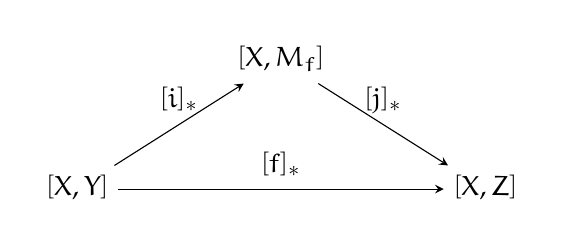
\begin{tikzpicture}
  \matrix (m) [matrix of math nodes,row sep=3em,column sep=4em,minimum width=2em]
  {
     & {[X,M_f]} &\\
     {[X,Y]} &  & {[X,Z]} \\};
  \path[-stealth]
    (m-2-1) edge node [above] {$[f]_*$} (m-2-3)
    (m-2-1) edge node [above] {$[i]_*$} (m-1-2)
    (m-1-2) edge node [above] {$[j]_*$} (m-2-3);
\end{tikzpicture}
\end{center}

y como $j$ es equivalencia homotópica, la función $[j]_*$ es biyectiva. Por lo tanto, $[f]_*$ es biyectiva sí y solo si $[i]_*$ lo es. Del mismo modo, $f$ es una equivalencia débil si y sólo si lo es $i$. 

Esto nos dice que sin pérdida de generalidad podemos probar el enunciado en el caso de $i : Y \to Z$ la inclusión de un subespacio $Y$ en un espacio topológico $Z$.

Ahora, como por hipótesis $i$ induce isomorfismos en los grupos de homotopía, de la suceción exacta larga de pares
\begin{align*}
\dots \to \pi_n(Y,y) \xrightarrow{i_*} \pi_n(Z,y) \to \pi_n(Z,Y,y) \to \dots
\end{align*}
vemos que debe ser $\pi_n(Z,Y,y) = 0$ para todo $n \in N$ e $y \in Y$.	

Por lo tanto, si $g : X \to Z$ es una función continua, es una función de pares de $(X, \emptyset)$ a $(Z,Y)$. Por el $\paint{\text{Lema $2$}}$, sabemos entonces que existe $h : X \to Z$ continua tal que $h \simeq g$ y $h(X) \subset Y$. En consecuencia, correstringiendo $h$ a $Y$ vemos que
\begin{align*}
[i]_*\left([h|^Y]\right) = [ih|^Y] = [h] =  [g],
\end{align*}
lo que prueba la sobreyectividad de $i_*$.

Ahora veamos la inyectividad. Sean $h_0,h_1 : X \to Y$ funciones continuas tales que $ih_0 \simeq ih_1$ y veamos que $h_0$ y $h_1$ son homotópicas. Por hipótesis, sabemos que existe una homotopía $H : ih_0 \simeq ih_1$, que puede ser vista como una función de pares de $(X \times I, X \times \partial I)$ a $(Z,Y)$, ya que tanto $ih_0$ como $ih_1$ tienen imagen en $Y$. 

Una vez más, por el $\paint{\text{Lema $2$}}$ existe una función continua $K : (X \times I, X \times \partial I) \to (Z,Y)$ y una homotopía $\Gamma : K \simeq H$ relativa a $X \times \partial I$ tal que $K(X \times I) \subset Y$. En particular $H$ y $K$ coinciden en $X \times \partial I$, así que si $s \in \{0,1\}$ entonces
\begin{align*}
h_s(x) = H(x,s) = K(x,s)
\end{align*}
para todo $x \in X$. Por lo tanto la correstricción $K|^Y : X \times I \to Y$ de $K$ es una función continua que satisface $K_s = h_s$, y consecuentemente $h_0$ y $h_1$ son homotópicas.
\end{proof}

\begin{center}
$\paint{
\rule{400pt}{0.5pt}
}$
\vspace{10pt}
\end{center}

\begin{lemma}{3} Sea $n \in \N$ y $f : \Ss^{2n} \to \Ss^{2n}$ una funci\'on continua. Si $f$ no tiene puntos fijos, entonces $\deg f = -1$.
\end{lemma}
\begin{proof} Notemos que como la homolog\'ia de $\Ss^{2n}$ es trivial excepto en grado $0$ y $2n$, es
\begin{align*}
\lambda(f) &= \sum_{q \geq 0}(-1)^q \cdot \tr(H_nf) = \tr(H_0f) + (-1)^{2n}\tr(H_{2n}f)\\
& = 1 + (-1)^{2n}\deg f = 1 + \deg f.
\end{align*}
Como $f$ no tiene puntos fijos debe ser $\lambda(f) = 0$, lo que nos dice que $\deg f = -1$. 
\end{proof}

\begin{exercise}{1} Probar que $\Z_2$ es el \'unico grupo no trivial que puede actuar libremente en una esfera de dimensi\'on par.
\end{exercise}
\begin{proof} Sea $n \in \N$ y $G$ un grupo que act\'ua libremente en $\Ss^{2n}$. Esto es equivalente a que para cada $g \in G$ distinto de la unidad la funci\'on 
\begin{align*}
m_g : \ & \Ss^{2n} \rightarrow \Ss^{2n}\\
&x \longmapsto g \cdot x
\end{align*}
no tenga puntos fijos. Por el $\paint{\text{Lema $3$}}$ sabemos entonces que $\deg m_g = -1$ para todo $g \neq 1$. 

Si ahora tomamos $g,h \in G \setminus \{1\}$ tenemos que
\begin{align*}
\deg m_{gh} = \deg m_g \circ m_h = \deg m_g \cdot \deg m_h = (-1)^2 = 1,
\end{align*}
asi que el contrarrec\'iproco del $\paint{\text{Lema $3$}}$ dice que $m_{gh}$ tiene puntos fijos: como la acci\'on es libre, debe ser $gh = 1$. 

Dado que $G$ no es trivial, existe alg\'un elemento $g \in G \setminus \{1\}$. Si ahora $h \in G \setminus \{1\}$ es arbitrario, de $gh^{-1} = 1$ obtenemos $h = g$ para cualquier $h \neq 1$. Por lo tanto es $G = \{1,g\}$. y en consecuencia, $G \simeq \Z_2$.
\end{proof}

\begin{center}
$\paint{
\rule{400pt}{0.5pt}
}$
\vspace{10pt}
\end{center}

\begin{lemma}{4} Sea $G$ un grupo. Si $x \in \Z[G]$ es no nulo y $G$-invariante, entonces $G$ es finito y existe $k \in \Z$ tal que $x = k \cdot \sum_{g \in G} g$.
\end{lemma}
\begin{proof} Como $x \in \Z[G] \setminus \{0\}$, existen finitos elementos $g_1, \dots, g_n \in G$ y enteros $a_1, \dots, a_n$ con $a_1 \neq 0$ tales que
\begin{align*}
x = a_1g_1 + \dots + a_ng_n.
\end{align*}
Para cada $g \in G$, es
\begin{align}
a_1g_1 + \dots + a_ng_n = x = gg_1^{-1}x = a_1g + a_2gg_1^{-1}g_2 + \dots + a_ngg_1^{-1}g_n
\end{align}
así que por la unicidad de la escritura en combinaciones formales, necesariamente $g \in \{g_1, \dots, g_n\}$. 
Esto prueba que $G = \{g_1, \dots, g_n\}$, y en particular $G$ resulta finito. 

Ahora, si para cada $i \in \nat{n}$ ponemos $g = g_i$ en la igualdad $\paint{(1)}$, se tiene que
\begin{align*}
a_1g_1 + \dots + a_ng_n = a_1g_i + \dots + a_ng_ig_1^{-1}g_n.
\end{align*}
Una vez más, por la unicidad de la escritura existe $k := a_1 \in \Z$ tal que $k = a_1 = \dots = a_n$ y consecuentemente
\begin{align*}
x = a_1g_1 + \dots a_ng_n = kg_1 + \dots kg_n = k \cdot \sum_{g \in G}g.
\end{align*}
\end{proof}

\begin{exercise}{5} Probar que $\operatorname{cd}(G) = 0$ si y sólo si $G$ es el grupo trivial.
\end{exercise}
\begin{proof} Una implicación es clara: si $G = 1$, un $\Z[1]$-módulo es simplemente un $\Z$ módulo, y entonces la sucesión
\begin{align*}
0 \to \Z \xrightarrow{id} \Z \to 0
\end{align*} 
es una resolución libre (en particular, proyectiva) de $\Z$ como $\Z[1]$-módulo trivial que tiene longitud cero. 

Recíprocamente, supongamos que existe una resolución proyectiva
\begin{align*}
0 \to P_0 \xrightarrow{\eps} \Z \to 0
\end{align*}
de $\Z$ como $\Z[G]$-módulo trivial. En particular $\Z$ resulta un $\Z[G]$-módulo proyectivo y por lo tanto, el epimorfismo
\begin{align*}
r : \sum_{g \in G}k_g \cdot g  \in \Z[G] \mapsto \sum_{g\in G}k_g \in \Z
\end{align*}
tiene una sección $s : \Z \to \Z[G]$. Como la acción de $G$ en $\Z$ es trivial, es
\begin{align*}
g \cdot s(1) = s(g \cdot 1) = s(1)
\end{align*}
para cada $g \in G$, y además $s(1) \neq 0$ pues al ser sección $s$ es inyectiva. Esto dice que $s(1)$ es no nulo y $G$-invariante, así que por el $\paint{\text{Lema $4$}}$ existe $k \in\Z$ tal que $s(1) = k \cdot \sum_{g \in G}g$. 

Aplicando $r$ se obtiene
\begin{align*}
1 = rs(1) = r\left(k \cdot \sum_{g \in G}g\right) = k \cdot \sum_{g \in G}1 = k |G|,
\end{align*}
lo que implica $|G| = k = 1$. Por lo tanto, necesariamente $G$ es el grupo trivial.
\end{proof}

\end{document}
